\subsection{Simulation model}
Fixing the problem in section 2.1 is not straight forward: swapping the two checks would
break other scenarios (\texttt{e.g.} M1 is due just after the \texttt{ElectionTimeout}).
The only definitive fix would have been rewriting the entire simulation system.
Given the use case and applications of Raft Scope we decided to limit the maximum speed to prevent such problems.

Network noise was integrated into the simulation and the state object, dropping each message with a probability
set by the user.

\subsection{Interaction}
\emph{Cluster membership changes} are an important part of a consensus protocol. Raft initially handled this with a procedure
called \emph{joint consensus} but Ongaro expanded on this matter in his Ph.D. thesis~\cite{ongaro2014consensus}(Chapter 4) with a new
simpler algorithm that only allows single server changes at a time (both removal and addition), however any arbitrary
change that could be expressed with joint consensus can be also managed with a series of single server changes that is easier to visualize.
Each configuration in the series must be committed before the next one can take place.
With the intention to clarify this series of changes, we added a \emph{cluster configuration changes queue}.
This queue keeps track of all the cluster reconfigurations submitted by the user while they are being processed.
The original dissertation is not clear on what action to take regarding pending configurations when leadership is lost.

A bug in the single server membership change algorithm was later found and discussed in the raft-dev mailing list~\cite{bug} which
could rewrite committed history. The bug occurred whenever leadership was lost and two pending configurations were happening
at the same time, submitted by different leaders. As described there, we implemented the fix by having leaders append a \texttt{NOOP} to their log.

We implemented a safety check for disruptive(removed) servers as described in section 4.2.3 of the author's thesis.
Servers, when removed, could disrupt cluster functionality by starting new elections whenever a pending change for their removal
is being processed. The fix makes servers ignore VoteRequest RPCs if they have received an heartbeat within
\texttt{MIN\_ELECTION\_TIMEOUT} from an active leader.

\subsection{Integrating the new features}
In order to allow transparent playback we modified the rendering phase in the main loop to take in account the possibility for
membership changes and automatic message drop due to network noise.
It was particularly challenging to determine when it is safe to remove a server
from the simulation: it is not correct to remove it when its corresponding configuration change is committed because
other servers, which have not yet received the entry, might still interact with it.
We decided to remove it when every other server has removed it from its \texttt{peers} list.

\subsection{Code reorganization}

\subsection{Interface}
For the timing issue discussed in Section~\ref{sec:internals} we limited the
simulation speed into a reasonable range.
The log table has been rewritten to support an infinite log and
now features also the auto scroll.
To avoid confusion the ``leader only'' fields in the state modal of the
follower servers have been hidden and a legend was added to explain the
otherwise cryptic symbols in the log table. Moreover, now, each log entry
is represented differently on the basis of its nature (\texttt{NOOP}, Config
change message, user value).
We obviously added controls for the feature we introduced in the Protocoll,
we thus added a slider to set the \emph{network noise}, a \emph{server add}
button and a voice to the context menu for server removal and finally
a new table to visualize the cluster configuration changes queue.
Besides that few minor bug were fixes.

\begin{figure*}[h]
    \centering
    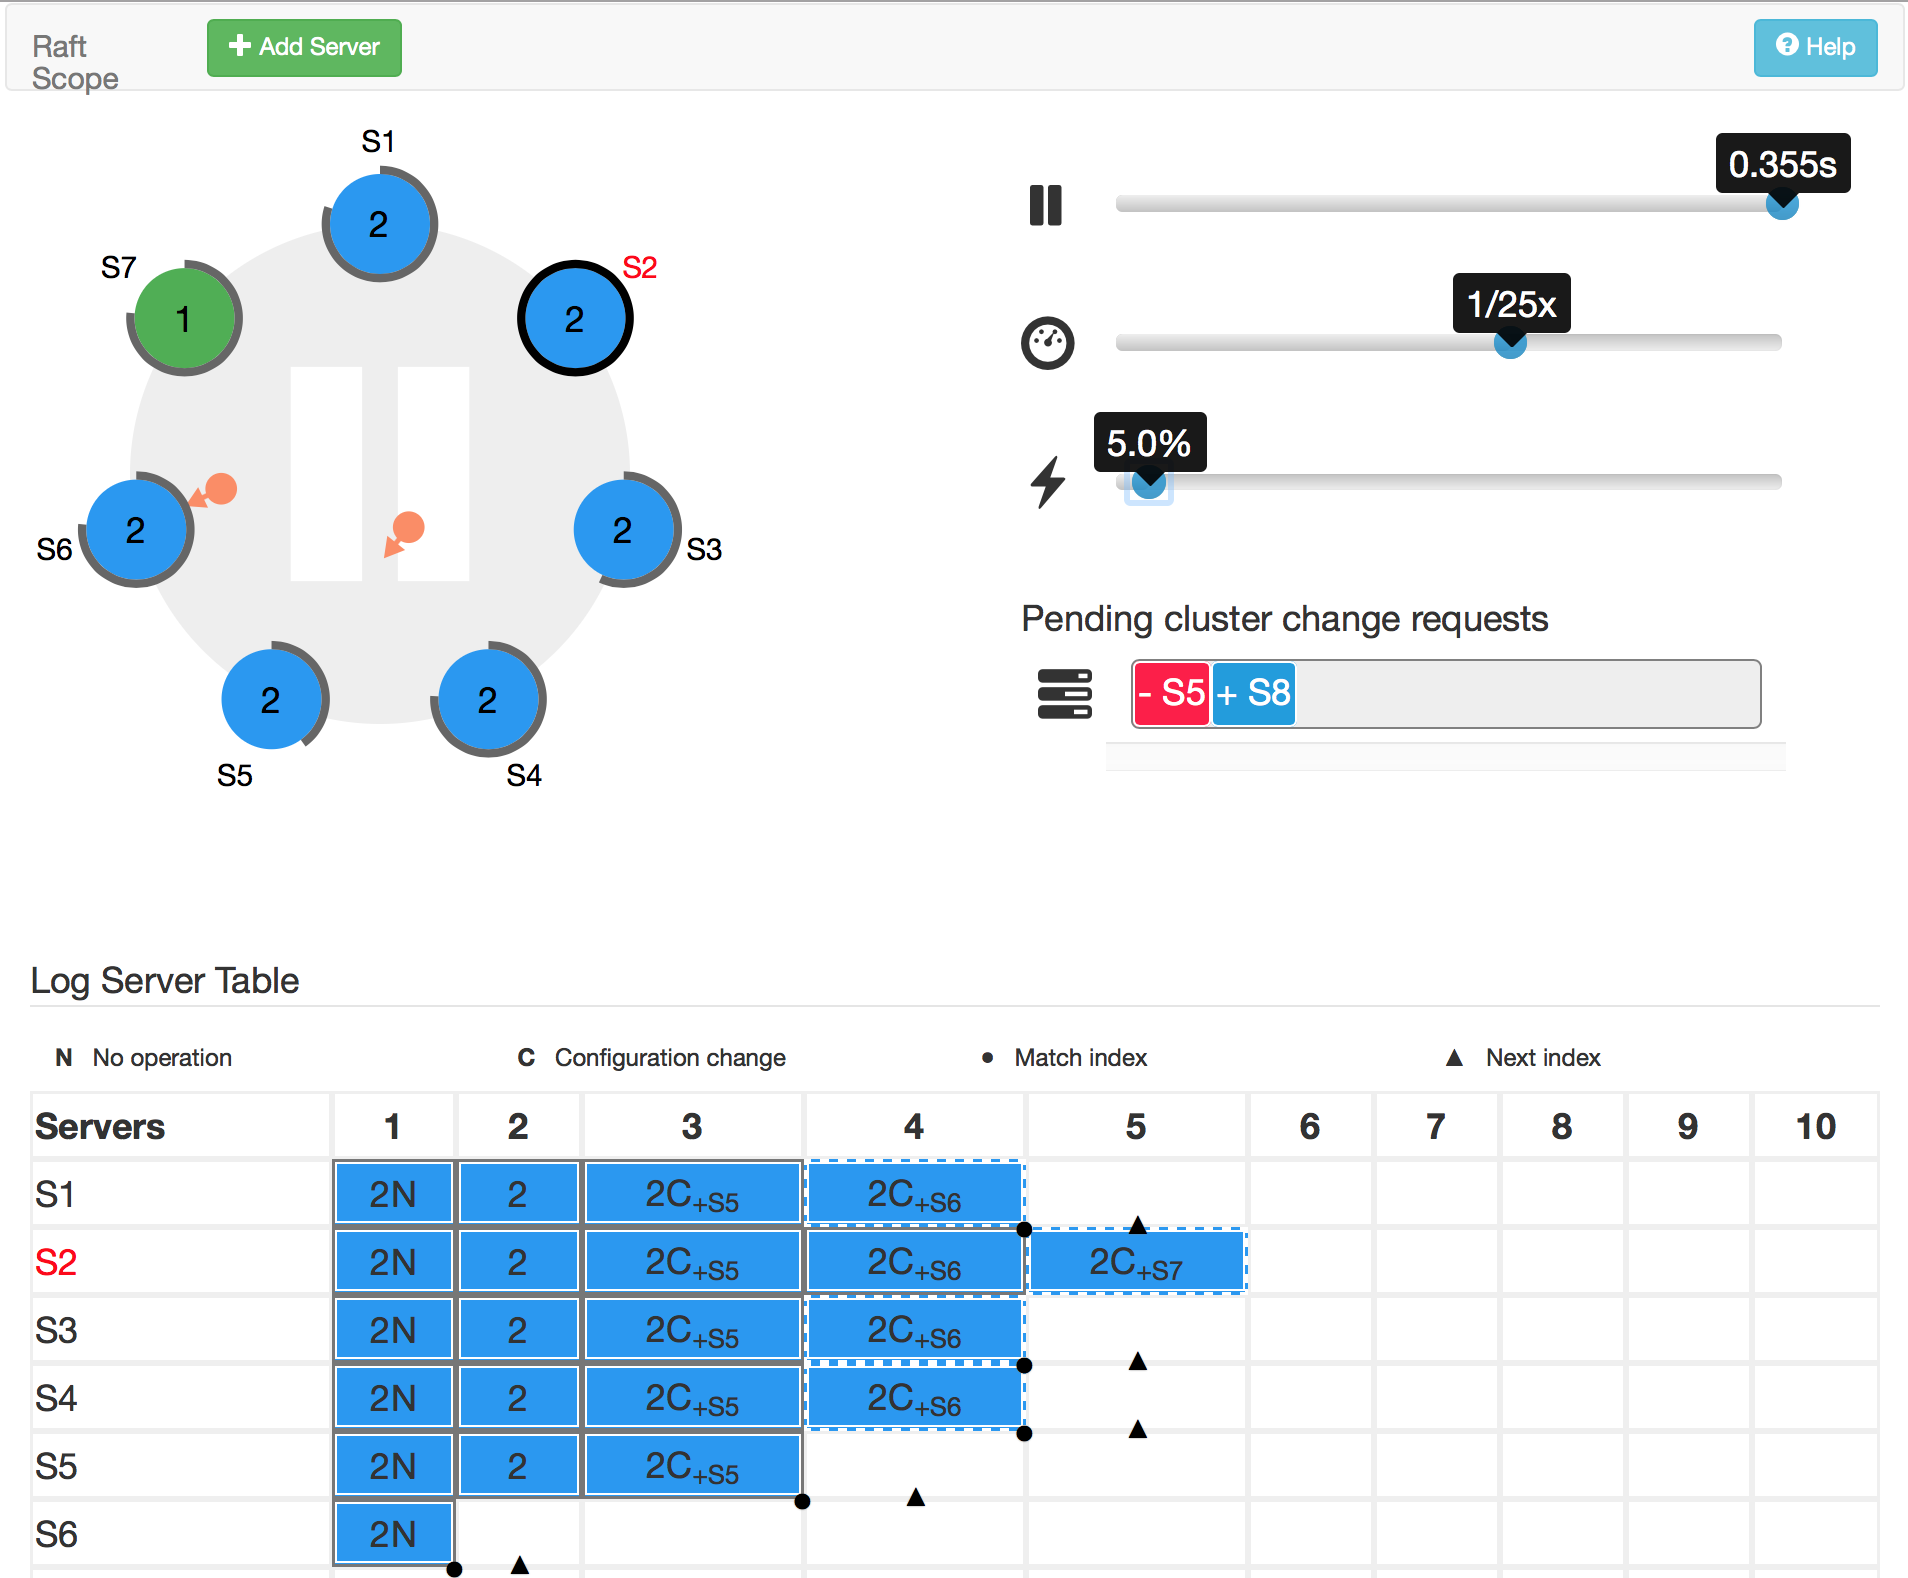
\includegraphics[width=0.9\linewidth]{our.png}
    \caption{Extended}\label{fig:final}
\end{figure*}

\subsection{Future work}
The \emph{leadership transfer extension} described in Section 3.10 of the thesis
was not implemented in the original Raft Scope or our work because it was not evaluated by the authors.